\section{Sistema C – Sistema Acesso ao Estacionamento}


O Sistema C tem como objetivo o controlo de um motor servo através de um comando de infravermelhos. O motor servo servirá como "portão". Deverá ser possível levantar e baixar o portão, assim como suspender o seu movimento. O programa apresenta ainda "multitasking" por "timer", para ser possível ler os valores do comando e alterar a posição do servo simultaneamente. O código elaborado foi o seguinte:


\begin{figure}[H]
    \centering
    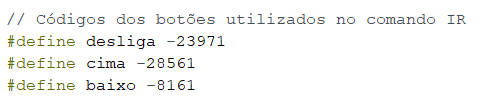
\includegraphics[scale=0.6]{images/codigo/sisC_codigosComando.png}
    \selectlanguage{portuguese}\caption{Código para o comando IR}
\end{figure}

\begin{figure}[H]
    \centering
    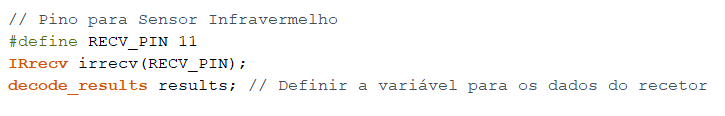
\includegraphics[scale=0.6]{images/codigo/sisC_definicaoRecetor.png}
    \selectlanguage{portuguese}\caption{Definição do sensor IR}
\end{figure}

\begin{figure}[H]
    \centering
    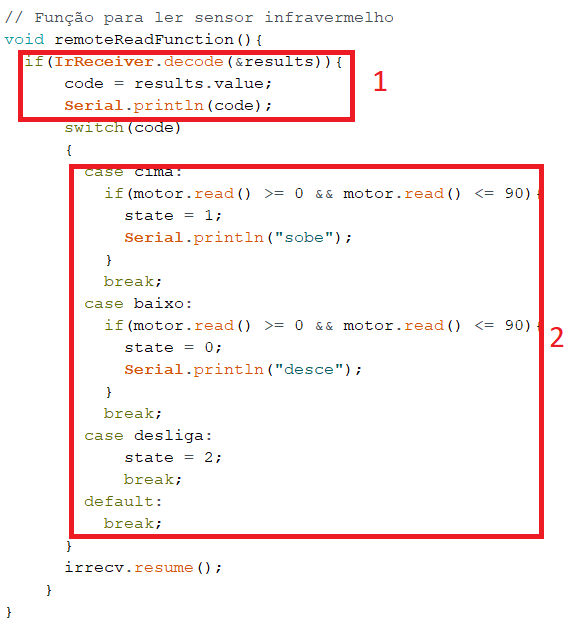
\includegraphics[scale=0.5]{images/codigo/sisC_remoteFunctionRead.png}
    \selectlanguage{portuguese}\caption{Função de leitura de valor do Sensor IR}
\end{figure}

\begin{itemize}
    \item 1 - Leitura do valor recebido pelo sensor de Infravermelhos.
    \item 2 - Caso o código seja um dos códigos definidos a variável "state" é alterada, esta variável serve para controlar o funcionamento do servo.
\end{itemize}

\begin{figure}[H]
    \centering
    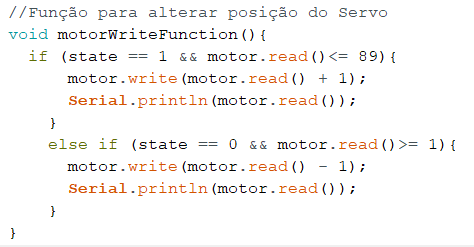
\includegraphics[scale=0.6]{images/codigo/sisC_servofunction.png}
    \selectlanguage{portuguese}\caption{Função para controlo do Servo}
\end{figure}

Esta função serve para alterar a posição do servo em 1 grau por cada iteração do programa, apenas no caso do "state" se encontrar igual a "0" ou "1".


\begin{figure}[H]
    \centering
    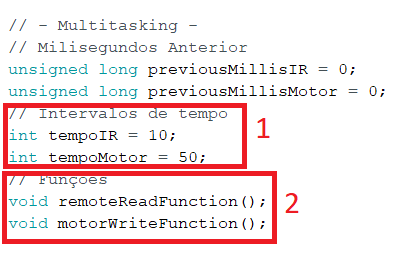
\includegraphics[scale=0.6]{images/codigo/sisC_definicaoMultitasking.png}
    \selectlanguage{portuguese}\caption{Definições para multitasking}
\end{figure}

\begin{itemize}
    \item 1 - Definidos os "delays" entre iterações de cada uma das funções.
    \item 2 - As funções para multitasking encontram-se aqui definidas.
\end{itemize}

\begin{figure}[H]
    \centering
    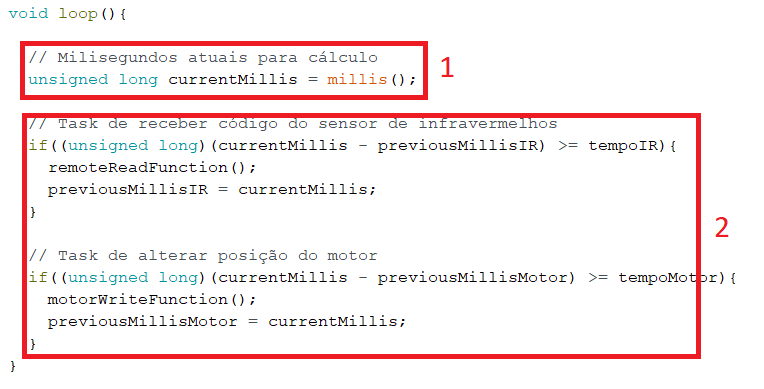
\includegraphics[scale=0.6]{images/codigo/sisC_multitaskingLoop.png}
    \selectlanguage{portuguese}\caption{Loop multitasking}
\end{figure}

\begin{itemize}
    \item 1 - São verficados sempre os milisegundos atuais para execução das funções por timer.
    \item 2 - Execução das funções apenas se se encotrarem no intervalo de tempo correto.
\end{itemize}